\section{Grundlagen} % (fold)
\label{sec:grundlagen}

	Für den durchgeführten Versuch stützen wir uns im Allgemeinen auf die folgenden Grundlagen des Gitterspektrographen und des CCD-Detektors.
	Die Theorie des Sonnenspektrums soll hier nur angerissen werden, da sie den Rahmen dieses Protokolls sprengen würde. 

	\subsection{Gitterspektrograph} % (fold)
	\label{sub:gitterspektrograph}

		\begin{figure}
			\center
			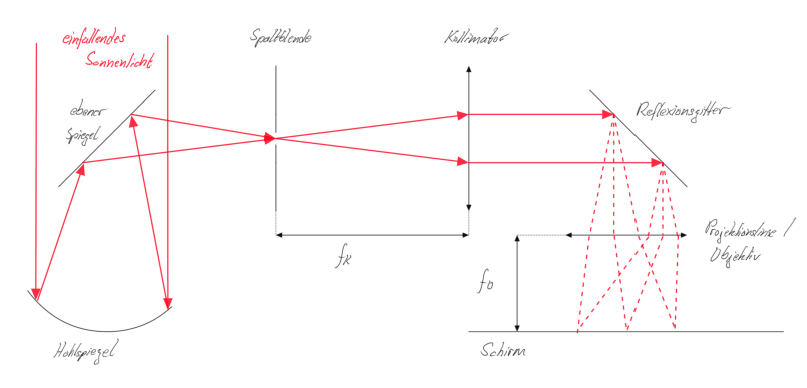
\includegraphics[scale=0.55]{skizzen/skizze-1.png}
			\caption{Skizze zum Aufbau des verwendeten Gitterspektrographen \\ $f_\mathrm{K}\ldots$Brennweite Kollimator \\ $f_\mathrm{O}\ldots$Brennweite Objektiv}
			\label{fig:skizze-spektrograph}
		\end{figure}

		Der grundsätzliche Aufbau des im Versuch verwendeten Gitterspektrographen ist in Abbildung \ref{fig:skizze-spektrograph} gezeigt.
		Hierbei wird das Sonnenlicht durch einen Hohlspiegel gebündelt und  durch eine Spaltblende zum Kollimator weitergeleitet.
		Durch den Spalt werden die Anteile des Lichts herausgefiltert, die nicht parallel zum Hohlspiegel eingefallen sind.
		Im Anschluss wird nun dieses divergierende Strahlenbündel mithilfe des Kollimators in ein rein paralleles Lichtbündel umgewandelt.
		Dieses trifft dann auf das Reflexionsgitter, welches wie ein typisches Gitter wirkt.
		Das Licht wird mit sich selbst interferieren, wodurch Beugungsmuster entstehen.
		Für große Entfernungen des Schirm interferieren näherungsweise parallele Strahlen miteinander.
		Die auftretenden Phänomene sind damit vergleichsweise leicht durch die Fraunhofer-Beugung berechenbar.
		Der Aufbau befindet sich jedoch in einem relativ kleinen geschlossenen System.
		Um die Bedingung, dass parallele Strahlen interferieren, dennoch nicht zu verletzen, werden durch eine Projektionslinse (auch Objektiv) parallel verlaufende Strahlen in einem Punkt auf dem Schirm fokussiert.
		Der Schirm zeigt also gerade die Spektrallinien des einfallendes Lichtes.

		Für den Abstand $x(n,\lambda)$ von der nullten Ordnung der Spektrallinie $n$.Ordnung mit Wellenlänge $\lambda$ ergibt sich dann näherungsweise
		\[ x(n,\lambda) = \frac{s}{g}n\lambda \]
		Dabei beschreibt $s$ den Abstand vom Gitter zum Schirm und $g$ die Gitterkonstante.
		Für das Auflösungsvermögen folgt dann
		\[ \frac{\lambda}{\Delta\lambda(n)} = \frac{x(n,\lambda)}{\Delta x(n,\lambda)} = nN \]
		wenn $N$ die Anzahl der beleuchteten Spalte am Reflexionsgitter beschreibt.

		Alle Berechnungen beruhen darauf, dass es sich um einen idealen Spektrographen handelt.
		Das heißt vor Allem, dass dabei die Spaltbreite der Spaltblende als gegen Null tendierend angenommen wird.
		Dies kann im Allgemeinen allerdings nicht realisiert werden, da sonst die Lichtintensität zu klein wäre.
		Aus diesem Grund wird das eigentliche Auflösungsvermögen stark durch die Spaltbreite bestimmt.
		Jede Spektrallinie ist dann eine Abbildung des Spalts.
	
	% subsection gitterspektrograph (end)

	\subsection{CCD-Detektor} % (fold)
	\label{sub:ccd_detektor}

		Um die Spektrallinien am Spektrograph messen zu können, wird der in Abbildung \ref{fig:skizze-spektrograph} beschriebene Schirm durch einen CCD-Detektor ersetzt.
		CCD-Detektoren bestehen aus einer Matrix lichtempfindlicher Fotodioden.
		Eine einfache Darstellung ist in Abbildung \ref{fig:schema-ccd} sichtbar.
		Einfallendes Licht überträgt durch den inneren photoelektrischen Effekt seine Energie auf die Elektronen der Halbleiter. 
		Dabei entstehen gleichzeitig negativ geladene freie Elektronen und positiv geladene \glqq Löcher\grqq, die sich aufgrund einer angelegten Spannung voneinander trennen. 
		Die Ladungen fließen jedoch nicht wie bei einer normalen Fotodiode sofort nach außen ab, sondern werden in der Speicherzelle selbst, in einem sogenannten Potentialtopf gesammelt, der wie ein Kondensator Ladungen speichert. 
		Die Ladungsmenge ist dabei proportional zur eingestrahlten Lichtmenge, wenn rechtzeitig ausgelesen wird, bevor die Leerlaufspannung der Fotodiode erreicht ist.
		Nach der Belichtung werden die Ladungen schrittweise verschoben, bis sie schließlich als Ladungspakete, eines nach dem anderen, den Ausleseverstärker erreichen. 
		Es wird eine von der Ladung und somit der Lichtmenge abhängige elektrische Spannung ausgegeben.
		Das Ausgangssignal des Sensors ist somit seriell.
		Durch Anwendung dieser Technik reicht es, bei der technischen Herstellung des CCD-Sensors einen Ausleseverstärker für die gesamte Matrix von Fotodioden zu verwenden.

		\begin{figure}
			\center
			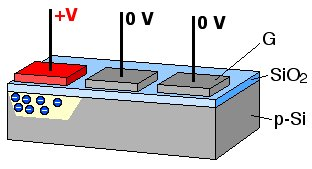
\includegraphics[scale=0.8]{referenzen/CCD_charge_transfer_animation.jpg}
			\caption{Schema eines CCD-Sensors (Quelle:\\ https://de.wikipedia.org/wiki/CCD-Sensor\#/media/File:CCD\_charge\_transfer\_animation.gif)}
			\label{fig:schema-ccd}
		\end{figure}

		Fotodioden eines CCD-Sensors können rechteckig, quadratisch oder polygonal sein, mit Kantenlängen von $1.4\unit{$\mu$m}$ bis über $20\unit{$\mu$m}$.
		Je größer die Fläche der Pixel, desto höher sind die Lichtempfindlichkeit und der Dynamikumfang, desto kleiner ist aber, bei gleicher Sensorgröße, die Bildauflösung.
		Bei Überbelichtung können Ladungen aus dem Potentialtopf einer Zelle in die Nachbarzellen übertreten.
		Die Messung von hohen Lichtintensitäten ist damit begrenzt.
		Abhilfe schaffte während des Versuches ein Papierfilter und die Einstellung einer kürzeren Belichtungszeit.

		Um nun mit dem CCD-Detektor auch Abstände oder Positionen messen zu können, muss ein bereits bekanntes Spektrum aufgenommen werden.
		So lassen sich dann mithilfe charakteristischer Spektrallinien die Skalierung $\alpha$ (Wellenlängenzunahme pro Pixel) und das Offset $\beta$ (Wellenlänge des linken äußersten Pixel) bestimmen.
		Näherungsweise können alle Funktionen als linear angesehen werden.
		Seien nun für zwei Wellenlängen $\lambda_1, \lambda_2$ mit $\lambda_1 < \lambda_2$ die Position bzw. die Pixel $p_1,p_2$ der Spektrallinien gegeben.
		Dann ergibt sich
		\begin{alignat*}{3}
			\alpha &= \frac{\lambda_2 - \lambda_1}{p_2 - p_1} \\
			\beta &= \lambda_1 - \alpha p_1
		\end{alignat*}
		Für die Wellenlänge eines beliebigen Pixels folgt dann, wenn alle Einstellungen am CCD-Detektor und am Spektrographen konstant bleiben
		\[ \lambda(p) = \alpha p + \beta \]
		Für gewisse Einstellungen und untersuchte Bereiche könnte diese Näherung verletzt werden.
		Um dies zu untersuchen, werden die gerade angegebenen Kalibrierungen nicht nur mit zwei Spektrallinien, sondern mit Mehreren an verschiedenen Stellen durchgeführt.

		Zur Auswertung der Intensitäten von Spektrallinien oder anderen Peaks ist es notwendig systematische und zufällige Fehler des CCD-Detektors zu kennen oder zu bestimmen.
		Hierfür spielen vor Allem die Kenngrößen Biaslevel, Rauschen und Dunkelstrom eine wichtige Rolle.
		
		Um ein Spannungssignal für verschiedene Pixel vom CCD-Sensor zu erhalten, werden, die Ladungen seriell ausgelesen, indem man die Ladungen von Diode zu Diode verschiebt.
		Bei dieser Verschiebung entsteht ein systematischer Fehler und eine statistische Abweichung (auch Rauschen) für jeden Pixel.
		Nach Beendigung des Auslesevorgangs wird zu jedem erhaltenen Wert ein sogenanntes Offset hinzuaddiert.
		Das Biaslevel eines Pixels ist dann gerade dieses Offset plus der systematische Fehler.

		Treffen keine Photonen auf den CCD-Sensor, so werden dennoch in jeder Fotodiode weitere Elektronen freigesetzt.
		Dieser Effekt entsteht durch die temperaturbedingte Bewegung der Elektronen, welche durch die geringe Bandlücke im Halbleiter ausreicht die Potentialbarriere zu überwinden.
		Die Anzahl der Elektronen pro Zeiteinheit, die so entstehen, wird Dunkelstrom genannt.
		Er ist jedoch unabhängig vom Photoneneinfall bzw. der Lichtintensität und somit ein Fehler in der Aufnahme.

	% subsection ccd_detektor (end)

	\subsection{Sonnenspektrum} % (fold)
	\label{sub:sonnenspektrum}

		Das elektromagnetische Spektrum der Sonne hat die größte Intensität im Bereich des sichtbaren Lichts. 
		Abhängig von der Wellenlänge wird die Sonnenstrahlung von der Atmosphäre mehr oder weniger stark absorbiert. 
		Die an der Erdoberfläche eintreffende Intensität hängt zudem stark vom Wetter und vom Sonnenstand ab.
		Beispiele des Sonnenspektrums zeigen die im Anhang \ref{sec:beispiele_des_sonnenspektrums} sichtbaren Abbildungen \ref{fig:sonnenspektrum-1} und \ref{fig:sonnenspektrum-2}.
		Das Spektrum ist von etwa $140 \unit{nm}$ bis etwa $10 \unit{cm}$ näherungsweise das eines Schwarzen Strahlers bei einer Temperatur von knapp $6000 \unit{K}$, der Temperatur der Photosphäre.
		Im Bereich von naher Infrarotstrahlung bis ins UV enthält das Spektrum eine Vielzahl von Absorptionslinien, die sogenannten Fraunhoferlinien. 
		Sie entstehen durch Strahlungsabsorption in der Chromosphäre der Sonne.
	
	% subsection sonnenspektrum (end)

% section grundlagen (end)